
%%%%%%%%%%%%%%%%%%%%%%%%%%%%%%%%%%%%%%%%%
% Beamer Presentation
% LaTeX Template
% Version 1.0 (10/11/12)
%
% This template has been downloaded from:
% http://www.LaTeXTemplates.com
%
% License:
% CC BY-NC-SA 3.0 (http://creativecommons.org/licenses/by-nc-sa/3.0/)
%%%%%%%%%%%%%%%%%%%%%%%%%%%%%%%%%%%%%%%%%

%----------------------------------------------------------------------------------------
%	PACKAGES AND THEMES
%------------------------------------------------s----------------------------------------

\documentclass{beamer}

% salem colors
\definecolor{burntorange}{rgb}{0.968, 0.549, 0.114}
\definecolor{burntorangedark}{rgb}{0.486, 0.306, 0.102}
\definecolor{lightblue}{rgb}{0.161, 0.471, 1}
\definecolor{lightbluedark}{rgb}{0.125, 0.271, 0.510}

\definecolor{charcoal}{rgb}{0.21, 0.27, 0.31}
\definecolor{darkgray}{rgb}{0.3, 0.3, 0.3}
\definecolor{darkgrey}{rgb}{0.33, 0.33, 0.33}
\definecolor{cadmiumgreen}{rgb}{0.0, 0.42, 0.24}
\definecolor{brandeisblue}{rgb}{0.0, 0.44, 1.0}
\setbeamercolor{structure}{fg=darkgray}
\setbeamercolor{footline}{fg=darkgray}

\mode<presentation> {

\usepackage{amssymb, bm}
\usepackage{amsmath, amsfonts, amscd, epsfig, amssymb, amsthm, adjustbox}
\usepackage{textcomp}
\usepackage{graphicx}
\usepackage{setspace}
\usepackage{enumitem}
\setlist[itemize]{itemsep=9pt, label={--}}

\usepackage{anyfontsize}
\usepackage{tcolorbox}[most]
\usepackage{tikz}
\usepackage[T1]{fontenc}
\usepackage{booktabs}
\usepackage{colortbl}
\usepackage{multirow}
\usepackage{array}
\usepackage{longtable}
\usepackage{listings}
\usepackage{color}
\usepackage{bbold}
\pagecolor{white}
\usepackage{mathtools}
\newcolumntype{K}[1]{>{\centering\arraybackslash}p{#1}}
\newcolumntype{Q}[1]{>{\columncolor[gray]{0.8}\centering\arraybackslash}p{#1}}
\newcommand\eho{\stackrel{\mathclap{\small\mbox{$H_0$}}}{=}}


\newcommand\norm[1]{\left\lVert#1\right\rVert}
\newcommand\smalldp{\fontsize{9.4}{7.2}\selectfont}
\newcommand\smalldpp{\fontsize{8.5}{7.2}\selectfont}
\newcommand\smalldppgh{\fontsize{9.5}{7.2}\selectfont}
\newcolumntype{H}{>{\setbox0=\hbox\bgroup}c<{\egroup}@{}}
\newcommand{\X}{\mathbf{X}}

\usepackage{color}
\pagecolor{white}
\usepackage[final]{pdfpages}

\newcommand{\bo}[1]{\textcolor{burntorange}{#1}}
\newcommand{\bod}[1]{\textcolor{burntorangedark}{#1}}
\newcommand{\lb}[1]{\textcolor{lightblue}{#1}}
\newcommand{\lbd}[1]{\textcolor{lightbluedark}{#1}}
\newcommand{\dg}[1]{\textcolor{darkgray}{#1}}

\newcommand{\dbl}{\setstretch{1.25}}
\newcommand{\hlf}{\setstretch{1}}

\newcommand{\bl}{\color{lightblue}}
\newcommand{\rd}{\color{burntorange}}
\newcommand{\bk}{\color{black}}
\newcommand{\gr}{\color{green}}

\newcommand{\bb}{$\lb{{\small \bullet } }$ \hspace{0.5mm}}
\newcommand{\ba}{$\lb{{\small \rightarrow } }$ \hspace{0.5mm}}

\newcommand{\bs}[1]{\boldsymbol{#1}}
\newcommand{\mc}[1]{\mathcal{#1}}
\newcommand{\mr}[1]{\mathrm{#1}}
%\newcommand{\bm}[1]{\mathbf{#1}}
\newcommand{\ds}[1]{\mathds{#1}}

\newcommand{\bi}{\begin{itemize}}
\newcommand{\ib}{\end{itemize}}
\newcommand{\p}{\item}
\newcommand{\sk}{\vspace{.5cm}}

\newcommand{\sko}{\vspace{.1in}}
\newcommand{\skoo}{\vspace{.2in}}
\newcommand{\skooo}{\vspace{.3in}}
\newcommand{\hko}{\hspace{.1in}}
\newcommand{\hkoo}{\hspace{.2in}}
\newcommand{\hkooo}{\hspace{.3in}}

\newcommand{\gvn}{\; | \;}

\newcommand{\E}{\ds{E}}
\newcommand{\var}{\mr{var}}


% The Beamer class comes with a number of default slide themes
% which change the colors and layouts of slides. Below this is a list
% of all the themes, uncomment each in turn to see what they look like.
\usepackage{color}
\pagecolor{white}
\usepackage[final]{pdfpages}
\usetheme{default}

\setbeamertemplate{navigation symbols}{}
\setbeamertemplate{footline}[frame number]{}
\setbeamertemplate{footline}{}
 % To remove the navigation symbols from the bottom of all slides uncomment this line
}

\usepackage{graphicx} % Allows including images
\usepackage{booktabs} % Allows the use of \toprule, \midrule and \bottomrule in tables

%----------------------------------------------------------------------------------------
%	TITLE PAGE
%----------------------------------------------------------------------------------------

\setbeamertemplate{footline}{\scriptsize{\hfill\insertframenumber\vspace{-.2cm}\hspace*{.35cm}}} 
%\addtobeamertemplate{footline}{\hspace{4mm}\includegraphics[scale=0.006]{uchicago_shield} \vspace{-0.6cm}}{\vspace{1cm}}
\addtobeamertemplate{footline}{\vspace{-0.4cm}}{\vspace{0.5cm}}
\addtobeamertemplate{headline}{\vspace{2.5mm}\hspace{120mm}

\includegraphics[scale=0.05]{salem-S}\vspace{-8mm}
}
%\setbeamertemplate{frametitle}{{\vspace{3mm}}}


%
\includegraphics[scale=.5]{UTlogo.png} 

\title[]{\Large{Machine learning for causal inference} \vspace{5mm}}

%'\subtitle{}

\author{David Puelz}
\institute[] % Your institution as it will appear on the bottom of every slide, may be shorthand to save space
{

}
\date{} % Date, can be changed to a custom date

\begin{document}

{\setbeamertemplate{footline}{}
\setbeamertemplate{headline}{}
\begin{frame}[noframenumbering]
\vspace{12mm}
\centerline{
\includegraphics[scale=0.075]{salem-banner}}
\vspace{5mm}
\titlepage % Print the title page as the first slide
\end{frame}
}

%% Overview slide
%\begin{frame}
%\frametitle{Overview} % Table of contents slide, comment this block out to remove it
%\tableofcontents % Throughout your presentation, if you choose to use \section{} and \subsection{} commands, these will automatically be printed on this slide as an overview of your presentation
%\end{frame}

%---------------------------------------------------------------------------------------
%	PRESENTATION SLIDES
%----------------------------------------------------------------------------------------

%------------------------------------------------


%------------------------------------------------


\begin{frame}
	\frametitle{Outline}
	
	\vspace{8mm}
Regularized causal effect estimation (linear) \\
	$$$$
Regularized causal effect estimation (nonlinear) \\
\end{frame}



\begin{frame}

\sk\sk
	\dg{\large \bf Regularized causal effect estimation (\bo{linear})}
\end{frame}


\begin{frame}
\frametitle{Kale}

\sk
Suppose we're interested in the {\bf treatment effect} of dietary kale intake.  
\vfill
And want to know how effective it is at lowering cholesterol, which is our {\bf outcome variable}. 
\vfill
Unfortunately, we have only observational data (i.e., not a randomized study).
\vfill
\end{frame}

\begin{frame}
\frametitle{Kale intake predicts exercise}
Our bad luck, only gym-rats seem to eat much kale.  And exercise is known to lower cholesterol: the ``direct'' effect is {\bf confounded}.
\vfill
$$Y_i = \beta_0 + \alpha Z_i + \varepsilon_i,$$ 
\vfill
Because $\mbox{cov}(Z_i, \varepsilon_i) \neq 0$, we can write 
\vfill
$$Y_i = \beta_0 + \alpha Z_i + \omega Z_i + \tilde{\varepsilon}_i.$$ 
\vfill
Since $\mbox{cov}(Z_i, \tilde{\varepsilon}_i) = 0$, we mis-estimate $\alpha$ as $\alpha + \omega$.
\vfill
\end{frame}


\begin{frame}
\frametitle{We must ``adjust'' for weekly exercise}
The good news is, we can {\bf control} for weekly exercise, $X_i$, by including it in the regression:
\vfill 
$$Y_i = \beta_0 + \alpha Z_i + \beta X_i + \varepsilon_i.$$ 
\vfill
This ``clears out" the confounding: conditional on $X_i$, $\mbox{cov}(Z_i, \varepsilon_i) = 0$ and we're good to go.
\vfill
\begin{center}
{\bf But what if we don't know what we need to control for?}
\end{center}
\vfill
\end{frame}

\begin{frame}
\frametitle{The problem with the kitchen sink}

\sk
So what is wrong with just including anything we can think of in our regression?
\vfill
The problem is that we typically have finite data. The more things we add, the more variable (untrustworthy) our estimator will be.
\vfill
How do people deal with this in practice?
\vfill
\end{frame}

\begin{frame}
\frametitle{The ``con'' of econometrics (1983)}
\begin{center}
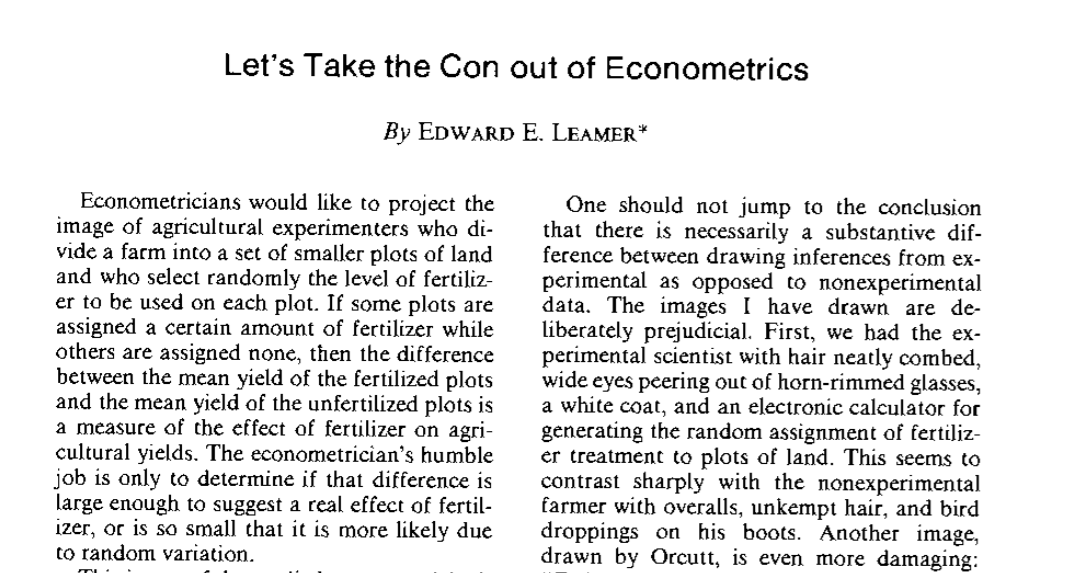
\includegraphics[width=4in]{figures/leamer.png}
\end{center}

\end{frame}

\begin{frame}
\frametitle{Enter ML and regularization}
It is well-known that shrinkage priors (e.g., point-mass priors) allow us to ``safely'' include many covariates in a regression (even more than our sample size!) \sk\sk

\bo{Classical stats} -- LASSO, ridge, stepwise selection ... \\ 
\bo{Bayesian stats} -- spike-and-slab \& horseshoe priors ...\\ 

\sk\sk
We have lots of theory backing this up, too.\sko
\begin{itemize}
\item bias-variance trade-off intuitions
\item  ``bet on sparsity" ideas
\end{itemize}
\vfill
%\begin{center}
%{\bf So we should control for as many things as possible and use our favorite shrinkage prior, right?}
%\end{center}
%\vfill
\end{frame}


\begin{frame}
\frametitle{The obvious approach}
$$Y_i = \beta_0 + \alpha Z_i + \beta X_i + \varepsilon_i.$$ 
\vfill
\begin{itemize}\addtolength{\itemsep}{1.25\baselineskip}
\item a flat prior on the treatment effect: $(\alpha, \sigma^2_{\varepsilon}) \propto 1/\sigma_{\varepsilon}$,
\item shrinkage prior on $\beta$ (e.g., a horseshoe prior).
\end{itemize}
\vfill

\begin{center}
{\bf And we're off to the races!}
\end{center}
\end{frame}



\begin{frame}
\frametitle{oops}
\begin{center}
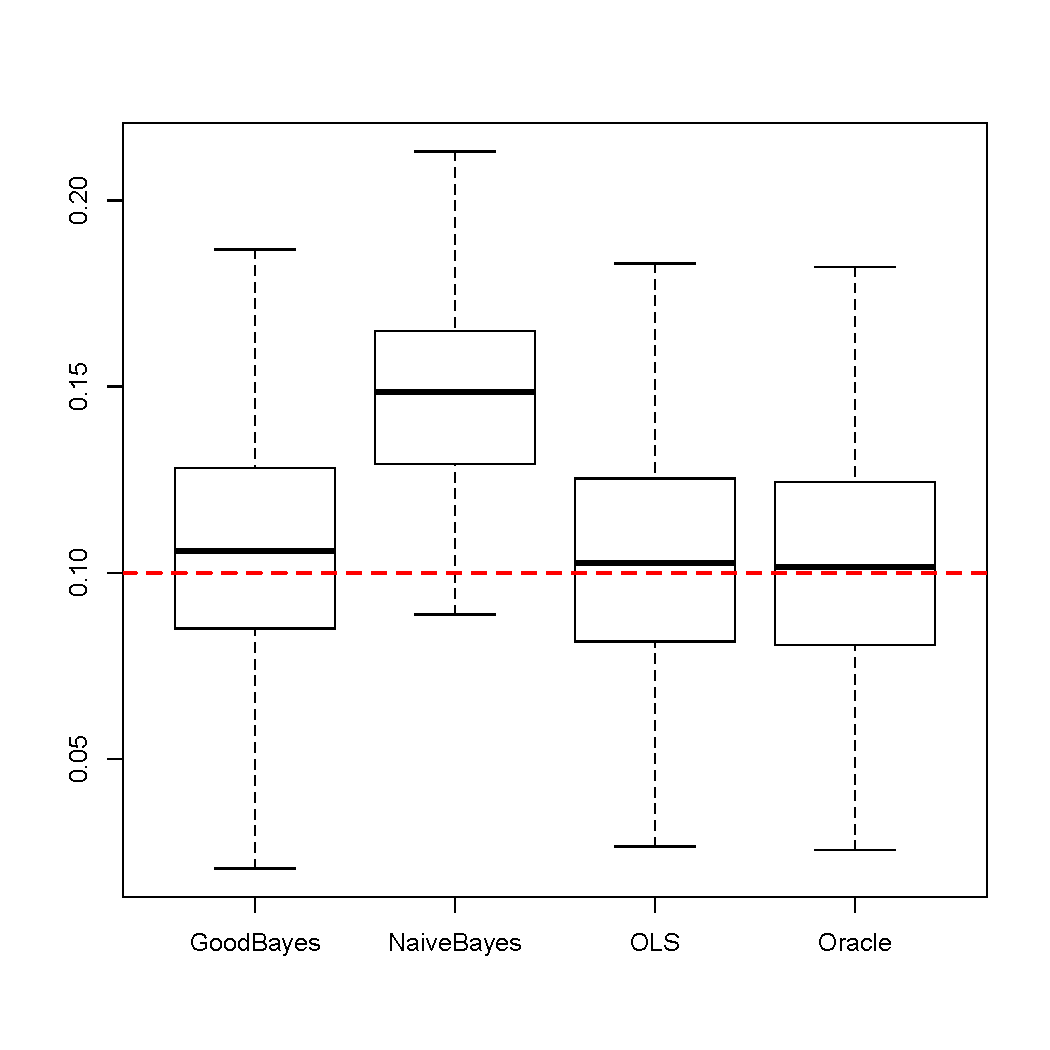
\includegraphics[width=2.5in]{figures/DominiciSims2_Estimates.pdf}
\end{center}
\vfill 
It turns out that this ``obvious'' approach is really bad at getting reasonable estimates of the treatment effect $\alpha$.
\vfill
\end{frame}


\begin{frame}
\frametitle{Bad bias versus good bias}
Assume that:
\begin{equation*}
	Z_i = \X_i^t\gamma + \epsilon_i.
\end{equation*}
\vfill
Now substitute a shrunk estimate, $\beta - \Delta$, in place of the true (unknown) $\beta$ vector:\sko
\begin{equation*} 
	Y_{i} = \alpha Z_{i} + \X_{i}^t(\beta - \Delta) + [\varepsilon_{i} + \X_{i}^t\Delta].
\end{equation*}\sko
This implies that $\varepsilon_{i}$ is taken to be $\varepsilon_{i} + \X_i^t\Delta$, which gives \sko
$$\mbox{cov}{( \X_i^t\gamma + \epsilon_i, \nu_{i} + \X_{i}^t\Delta)} \neq 0.$$ 

\sko
Biasing $\beta$ towards zero biases $\mbox{cov}(Z, \varepsilon)$ \bo{away from zero!}
\end{frame}

\begin{frame}
	\frametitle{Regularization-induced confounding (RIC)}
	
	This phenomenon biases inference in linear models, but it will also do the same  for anything else that uses regularization: \\\sk  
\small	
	$\bo{\bullet}$ \dg{Random forests}\\
	$\bo{\bullet}$ \dg{Neural nets}\\
	$\bo{\bullet}$ \dg{LASSO and ridge}\\
	$\bo{\bullet}$ \dg{all other ML methods!}\\
	
	
	 
\end{frame}


\begin{frame}
\frametitle{Our solution for the linear model}
\sk
\bo{Typical parameterization}
\begin{equation*}
	\begin{split}
	\text{Selection Eq.:} &\hspace{5mm}	Z = \X^t\gamma + \epsilon, \hspace{16.3mm} \epsilon \sim N(0,\sigma_{\epsilon}^{2}), 
		\\
		\text{Response Eq.:} &\hspace{5mm}	Y = \alpha Z + \X^t\beta + \nu, \hspace{5mm} \nu \sim N(0,\sigma_{\nu}^{2}).
	\end{split}
\end{equation*}
\end{frame}





\begin{frame}
\frametitle{Our reparameterization: a latent error approach}
\bo{We reparameterize as} 
\begin{equation*}
\begin{pmatrix}
\alpha\\
\beta +  \alpha \gamma\\
\gamma
\end{pmatrix} \rightarrow \begin{pmatrix}
\alpha \\
\beta_d\\
\beta_c
\end{pmatrix}.
\end{equation*}
which gives the new equations
\begin{equation*}
	\begin{split}
	\text{Selection Eq.:} &\hspace{5mm}	Z = \X^t\beta_c + \epsilon, \hspace{32.2mm} \epsilon \sim N(0,\sigma_{\epsilon}^{2}), 
		\\
		\text{Response Eq.:} &\hspace{5mm}	Y = \alpha(Z - \X^t\beta_c) + \X^t\beta_d + \nu, \hspace{5mm} \nu \sim N(0,\sigma_{\nu}^{2}).
	\end{split}
\end{equation*}
\begin{center}
\vspace{3mm}
{\bf We can now shrink $\beta_d$ and $\beta_c$  with impunity!}
\vspace{3mm}
\end{center}

{\small \dg{Note: This can also work by including $\hat{Z}$ as an unpenalized covariate with the original treatment $Z$.}}

\end{frame}


\begin{frame}
\frametitle{Variance reduction with minimal effect biasing}

\vspace{-8mm}
\begin{center}
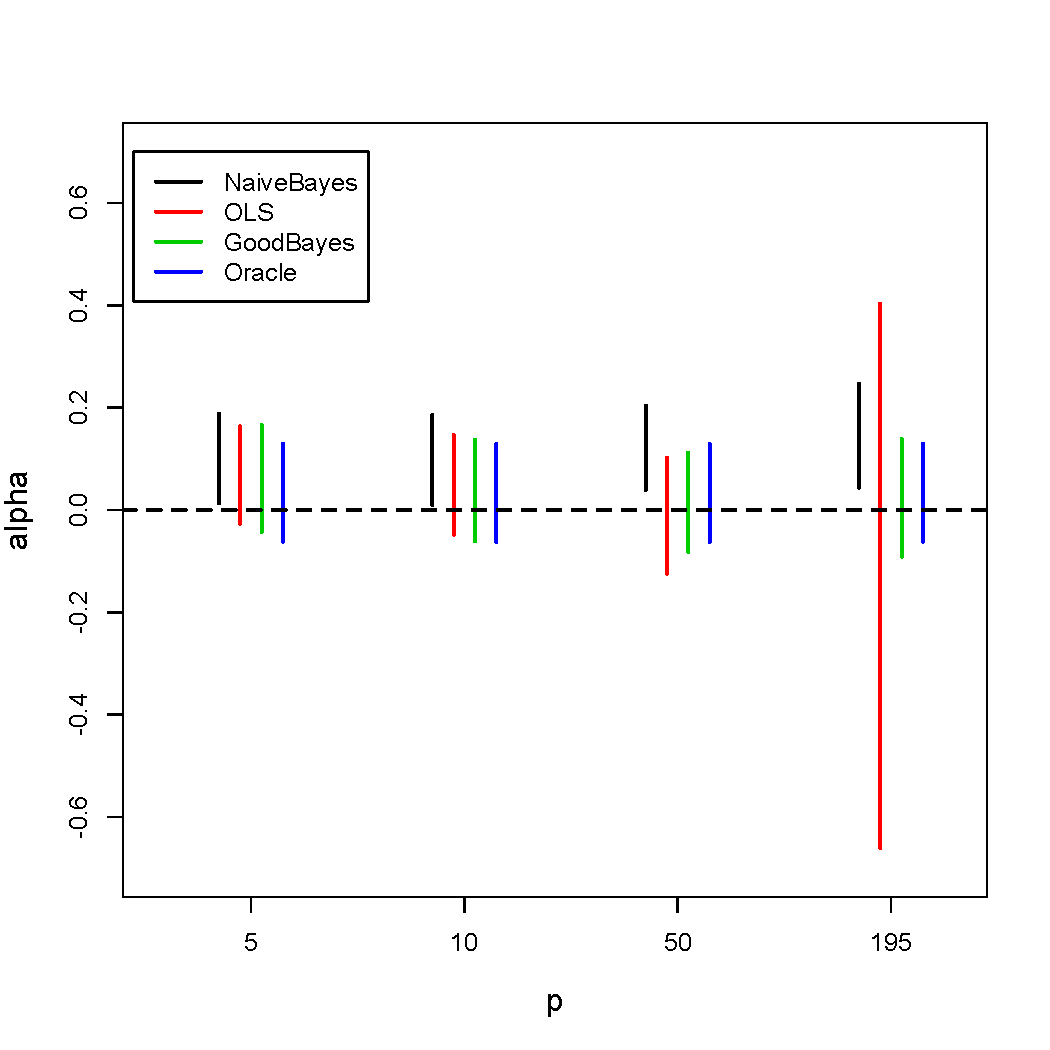
\includegraphics[width=2.75in]{figures/DominiciSims1_plot2.pdf}
\end{center}
\vspace{-5mm}
Eventually OLS is no good (too variable). The obvious (naive) approach breaks way before that!
\vfill
\end{frame}


\begin{frame}

\sk\sk
	\dg{\large \bf Regularized causal effect estimation (\bo{nonlinear})}
\end{frame}

\begin{frame}
	\frametitle{Moving from this ...}
\Large
$$Y = \beta_0 + \alpha Z + \beta X + \varepsilon$$ 	
	
\end{frame}


\begin{frame}
	\frametitle{To this!}
\Large
$$Y = f(X,Z) +  \varepsilon$$ 	

\sk
\pause
\small
${\dg{\rightarrow}}$ \normalsize default (supervised) framework for causal inference \\ \sko
${\dg{\rightarrow}}$ \normalsize a rich output that allows you to ask many questions
\end{frame}


\begin{frame}
	\frametitle{Conditional average treatment effect}
	
	Estimand of interest: \\ \sk
	
	\[\tau(\mathbf{x}_i) := E(Y_i|\mathbf{x}_i,Z_i=1) - E(Y_i|\mathbf{x}_i,Z_i=0)\] \\ \sk\sko
	
	So, treatment effect estimation is just \lb{response surface estimation}!
	
\end{frame}


\begin{frame}
	\frametitle{Conditional average treatment effect}
	
	Assuming mean zero additive errors: \\
	
$$Y_i = f(\mathbf{x}_i, Z_i) + \epsilon_i, \qquad \epsilon_i \sim N(0,\sigma^2)$$ \sko
 such that $$E(Y_i \mid \mathbf{x}_i,Z_i=z_i) = f(\mathbf{x}_i,z_i)$$

\sk

 Then our quantity of interest is
 $$\tau(\mathbf{x}_i) = f(\mathbf{x}_i,1) - f(\mathbf{x}_i,0)$$
\sk \vspace{-5mm}

\hspace*{20mm}\dg{\bf So, how do we regularize (model) $f$?}  

\end{frame}


\begin{frame}
	\frametitle{BART}
	
Bayesian Additive Regression Trees (\bo{BART}) from Chipman, George, \& McCulloch, (2008):

\sk
$$
y_i = f(\mathbf{x}_i) + \epsilon_i,\quad \epsilon_i\sim N(0, \sigma^2)
$$$$f(\mathbf{x}) = \sum_{h=1}^m g(\mathbf{x}, T_h, M_h)$$

\sk 
\dg{\small $\bullet$ Tree growth is probabilistic }\\
\dg{\small $\bullet$ Results in ensembles of smaller, simpler trees (\lb{regularization!}) }
	
\end{frame}


\begin{frame}
	\frametitle{Regression trees}
	
	\hspace*{-3mm}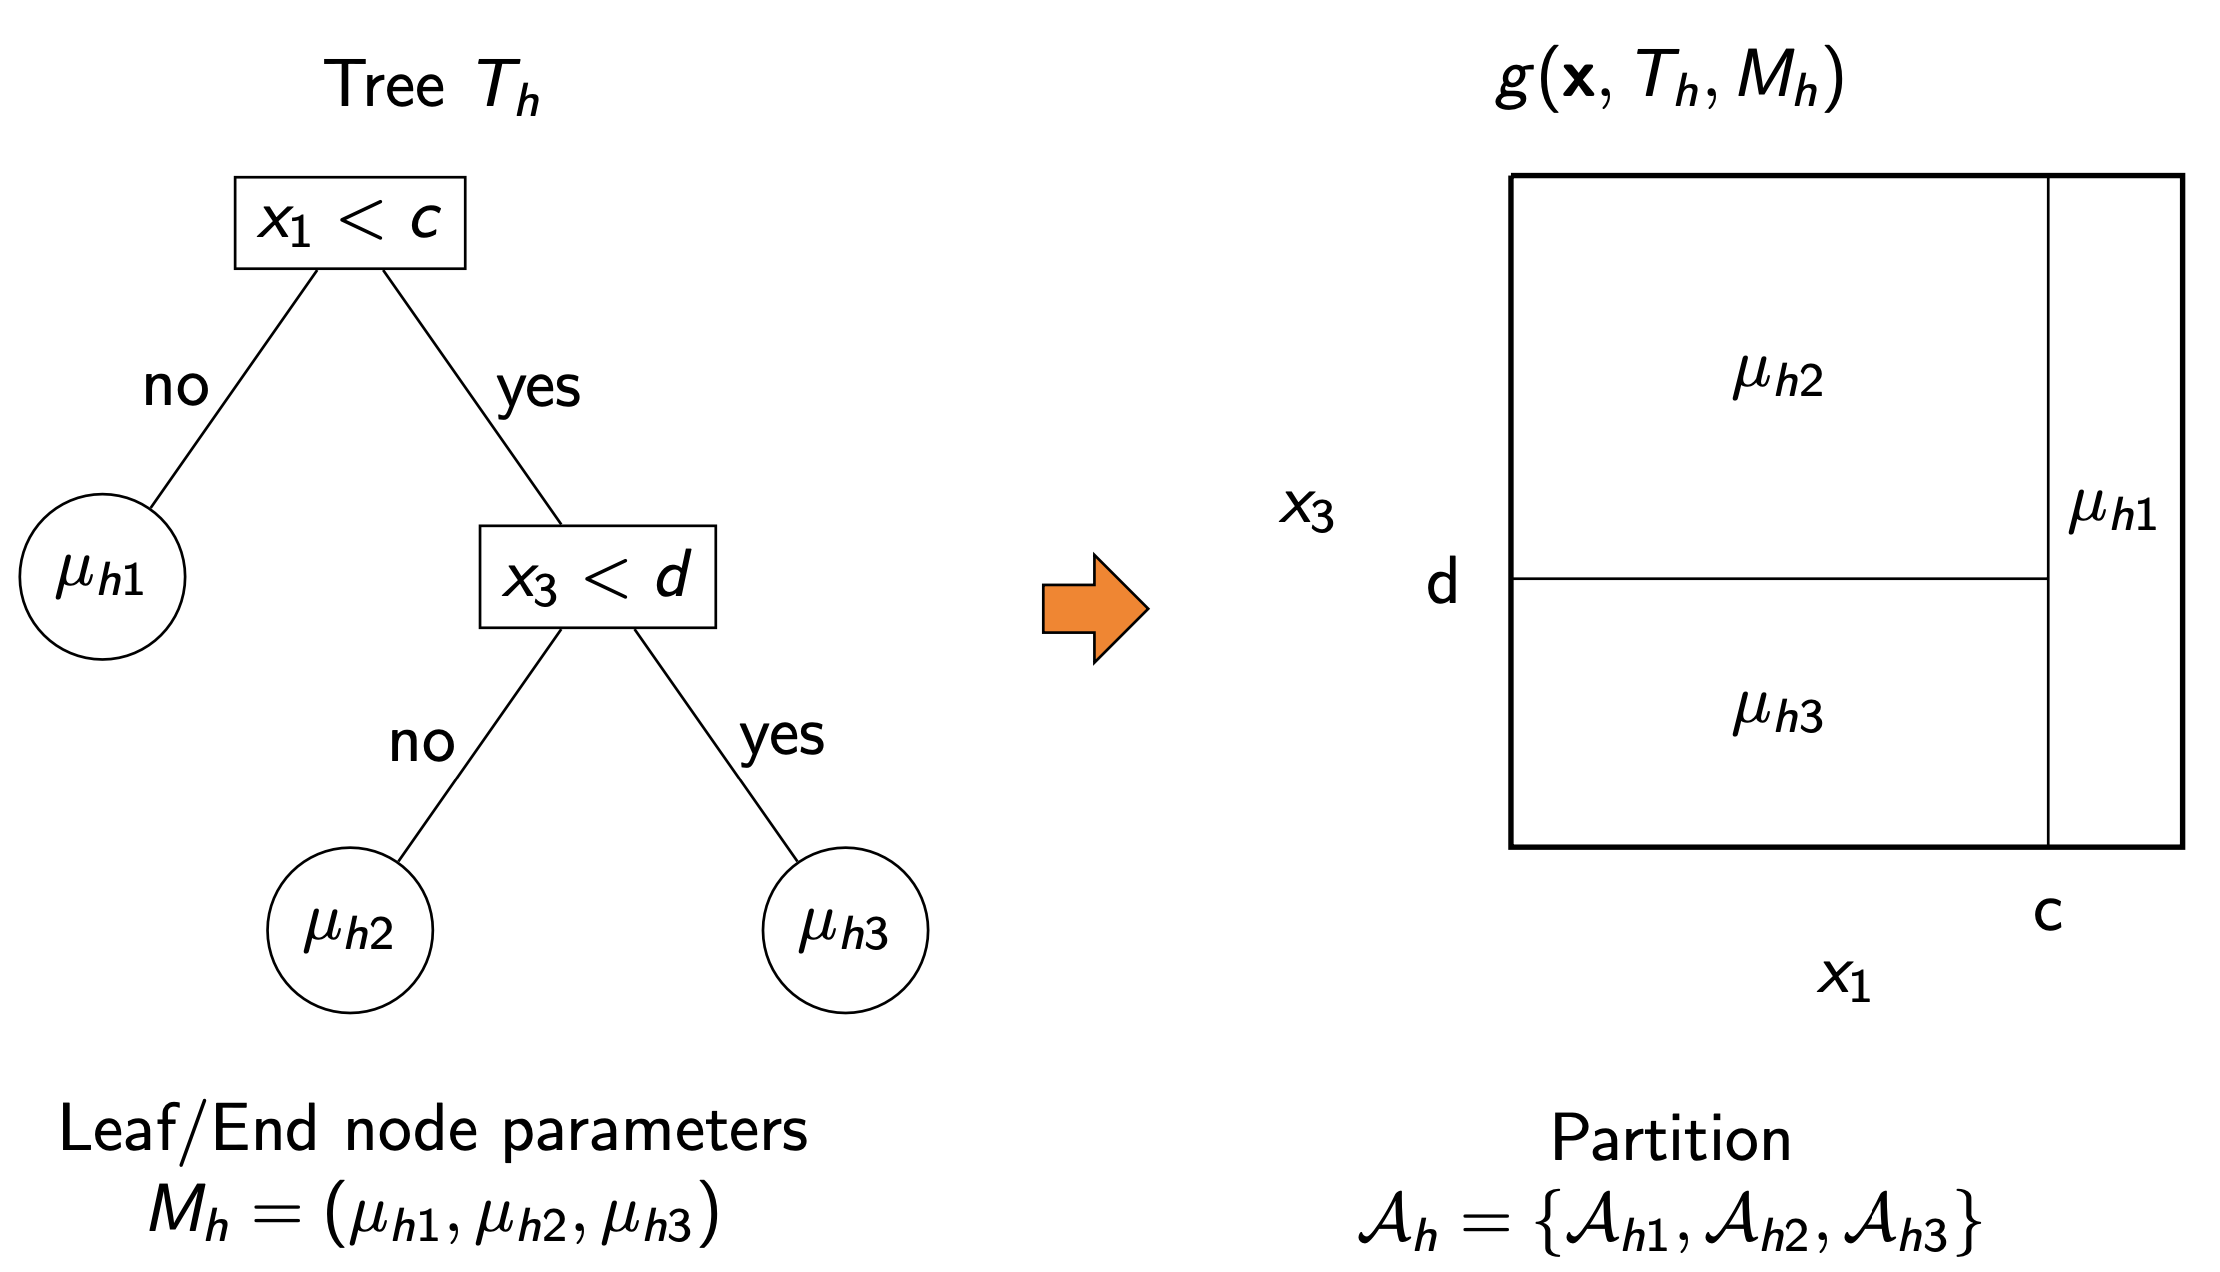
\includegraphics[scale=0.29]{figures/trees3} \vspace{1mm}

	\hspace*{25mm}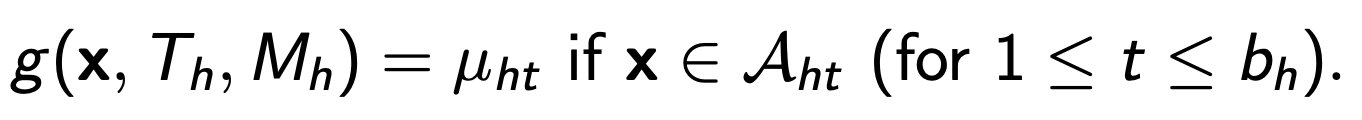
\includegraphics[scale=0.28]{figures/trees4}
	
\end{frame}


%\begin{frame}
%	\frametitle{Example BART fit}
%	
%
%	\hspace*{9mm}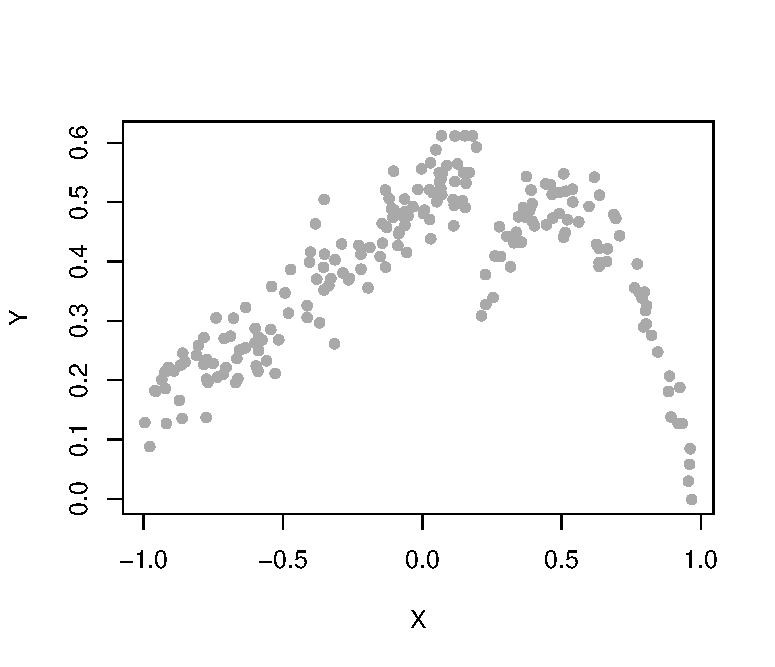
\includegraphics[scale=0.7]{figures/sim}
%	
%\end{frame}
%
%\begin{frame}
%	\frametitle{Example BART fit}
%%	\hspace*{9mm}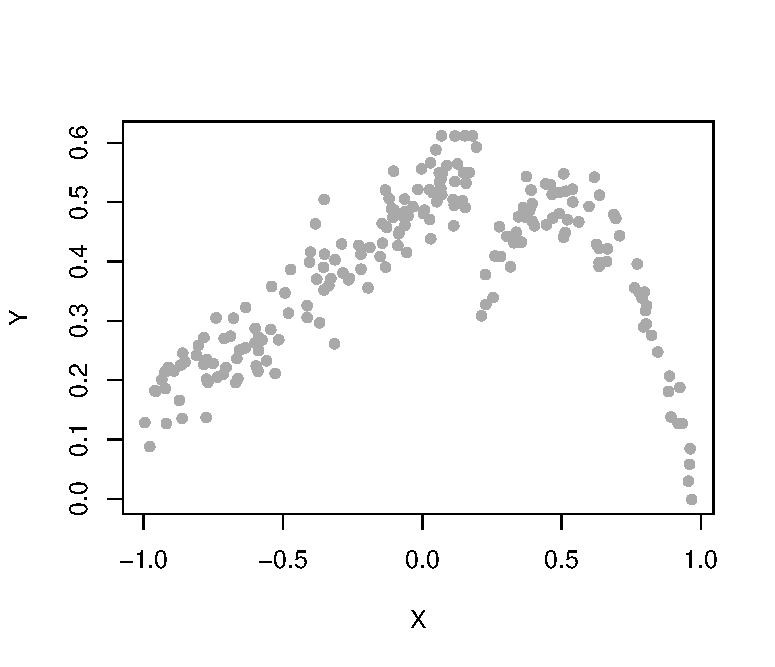
\includegraphics[scale=0.7]{figures/sim}	
%	\hspace*{9mm}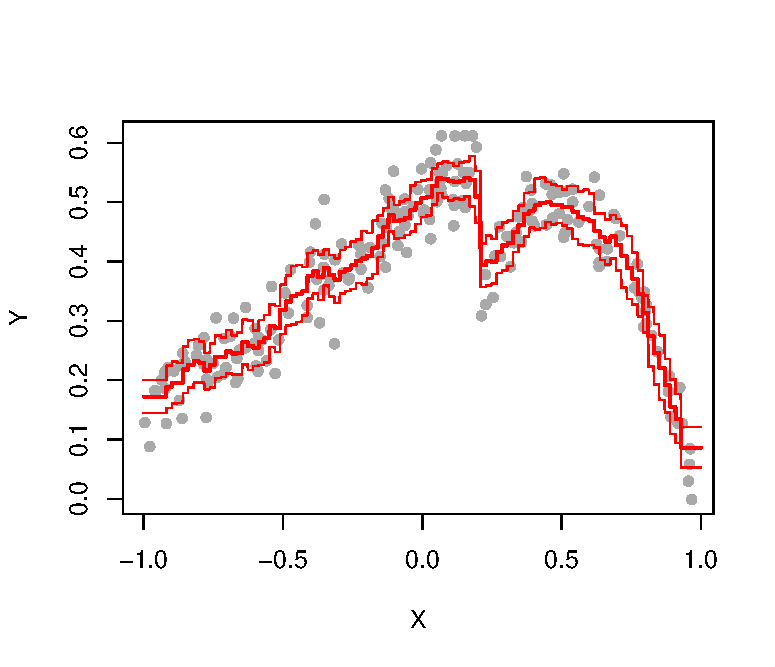
\includegraphics[scale=0.7]{figures/sim_bart.pdf}
%	
%\end{frame}

\begin{frame}
	\frametitle{Add in a treatment variable and go?}
Add treatment indicator as input variable (Hill, 2011): \\ \sk
$y_i = f(\mathbf{x}_i, \lb{z_i}) + \epsilon_i,\quad \epsilon_i\sim N(0, \sigma^2)$ \\ \sk
$f(\mathbf{x}, \lb{z}) = \sum_{h=1}^m g(\mathbf{x}, \lb{z}, T_h, M_h)$
	 
\sk \pause
\begin{center}
	\begin{tabular}{lcrc}
Prior & Bias & Coverage & RMSE\\
\hline
BART & 0.14& 31\% & 0.15\\
%Oracle BART & 0.00&98\% &0.05\\
%ps-BART & 0.06& 85\%&0.08
\hline
\end{tabular}
\end{center}

\sk
\bo{\bf Regularization-induced confounding (RIC), again!}
	
	
\end{frame}

\begin{frame}
	\frametitle{What do we do? {\small (borrow experience from regularized linear models)}}
	
	\bo{\bf Fix \#1} \dg{\small (ps-BART)}: Add in propensity $\hat{\pi}(\mathbf{x}) = P(Z=1 \mid \mathbf{x})$ as a covariate.
	
	$$y_i = f(\mathbf{x}_i, \lb{z_i},\lb{\hat{\pi}(\mathbf{x}_i)}) + \epsilon_i$$  \\ \sk\sk

	\bo{\bf Fix \#2} \dg{\small (BCF)}: Reparameterize to directly control regularization on prognostic and treatment effect functions.

	
	$$y_i = f(\mathbf{x}_i,\lb{z_i},\lb{\hat{\pi}(\mathbf{x}_i)}) + \epsilon_i$$
	$$\hspace*{16mm}= \mu(\mathbf{x}_i,\lb{\hat{\pi}(\mathbf{x}_i)}) + \tau(\mathbf{x}_i)\lb{z_i} + \epsilon_i$$
	
	\dg{\small Put independent BART priors on $\mu$ and $\tau$ and you're good to go!}
\end{frame}

\begin{frame}
	\frametitle{Propensity score BART}
	
	\begin{center}
\begin{tabular}{lcrc}
Prior & Bias & Coverage & RMSE\\
\hline
BART & 0.14& 31\% & 0.15\\
Oracle BART & 0.00&98\% &0.05\\
ps-BART & 0.06& 85\%&0.08 \\
\hline
\end{tabular}
\end{center}
\end{frame}

\begin{frame}
	\frametitle{ACIC 2017 {\small (data challenge for causal inference nerds)}}
	with BCF and causal RF (Wager and Athey): \\ \sk

{
% latex table generated in R 3.3.3 by xtable 1.8-2 package
% Sat Jun 23 10:11:47 2018
\begin{table}[ht]
\centering
\begin{tabular}{rrrr}
  \hline
 & Coverage & IL & Bias \\ 
  \hline
    BART & 0.81 & 0.040 & -0.0016  \\ 
  ps-BART & 0.88 & 0.038 & -0.0011  \\ 
BCF & 0.82 & 0.026 & -0.0009  \\ 
  Causal RF & 0.58 & 0.055 & -0.0155 \\
   \hline
\end{tabular}
\end{table}
}

\sk
{\small note that Wager and Athey's method also suffers from \bo{\bf RIC!}}
	
\end{frame}


\begin{frame}
	\frametitle{ACIC 2017 {\small (data challenge for causal inference nerds)}}
	
	\hspace*{-8mm}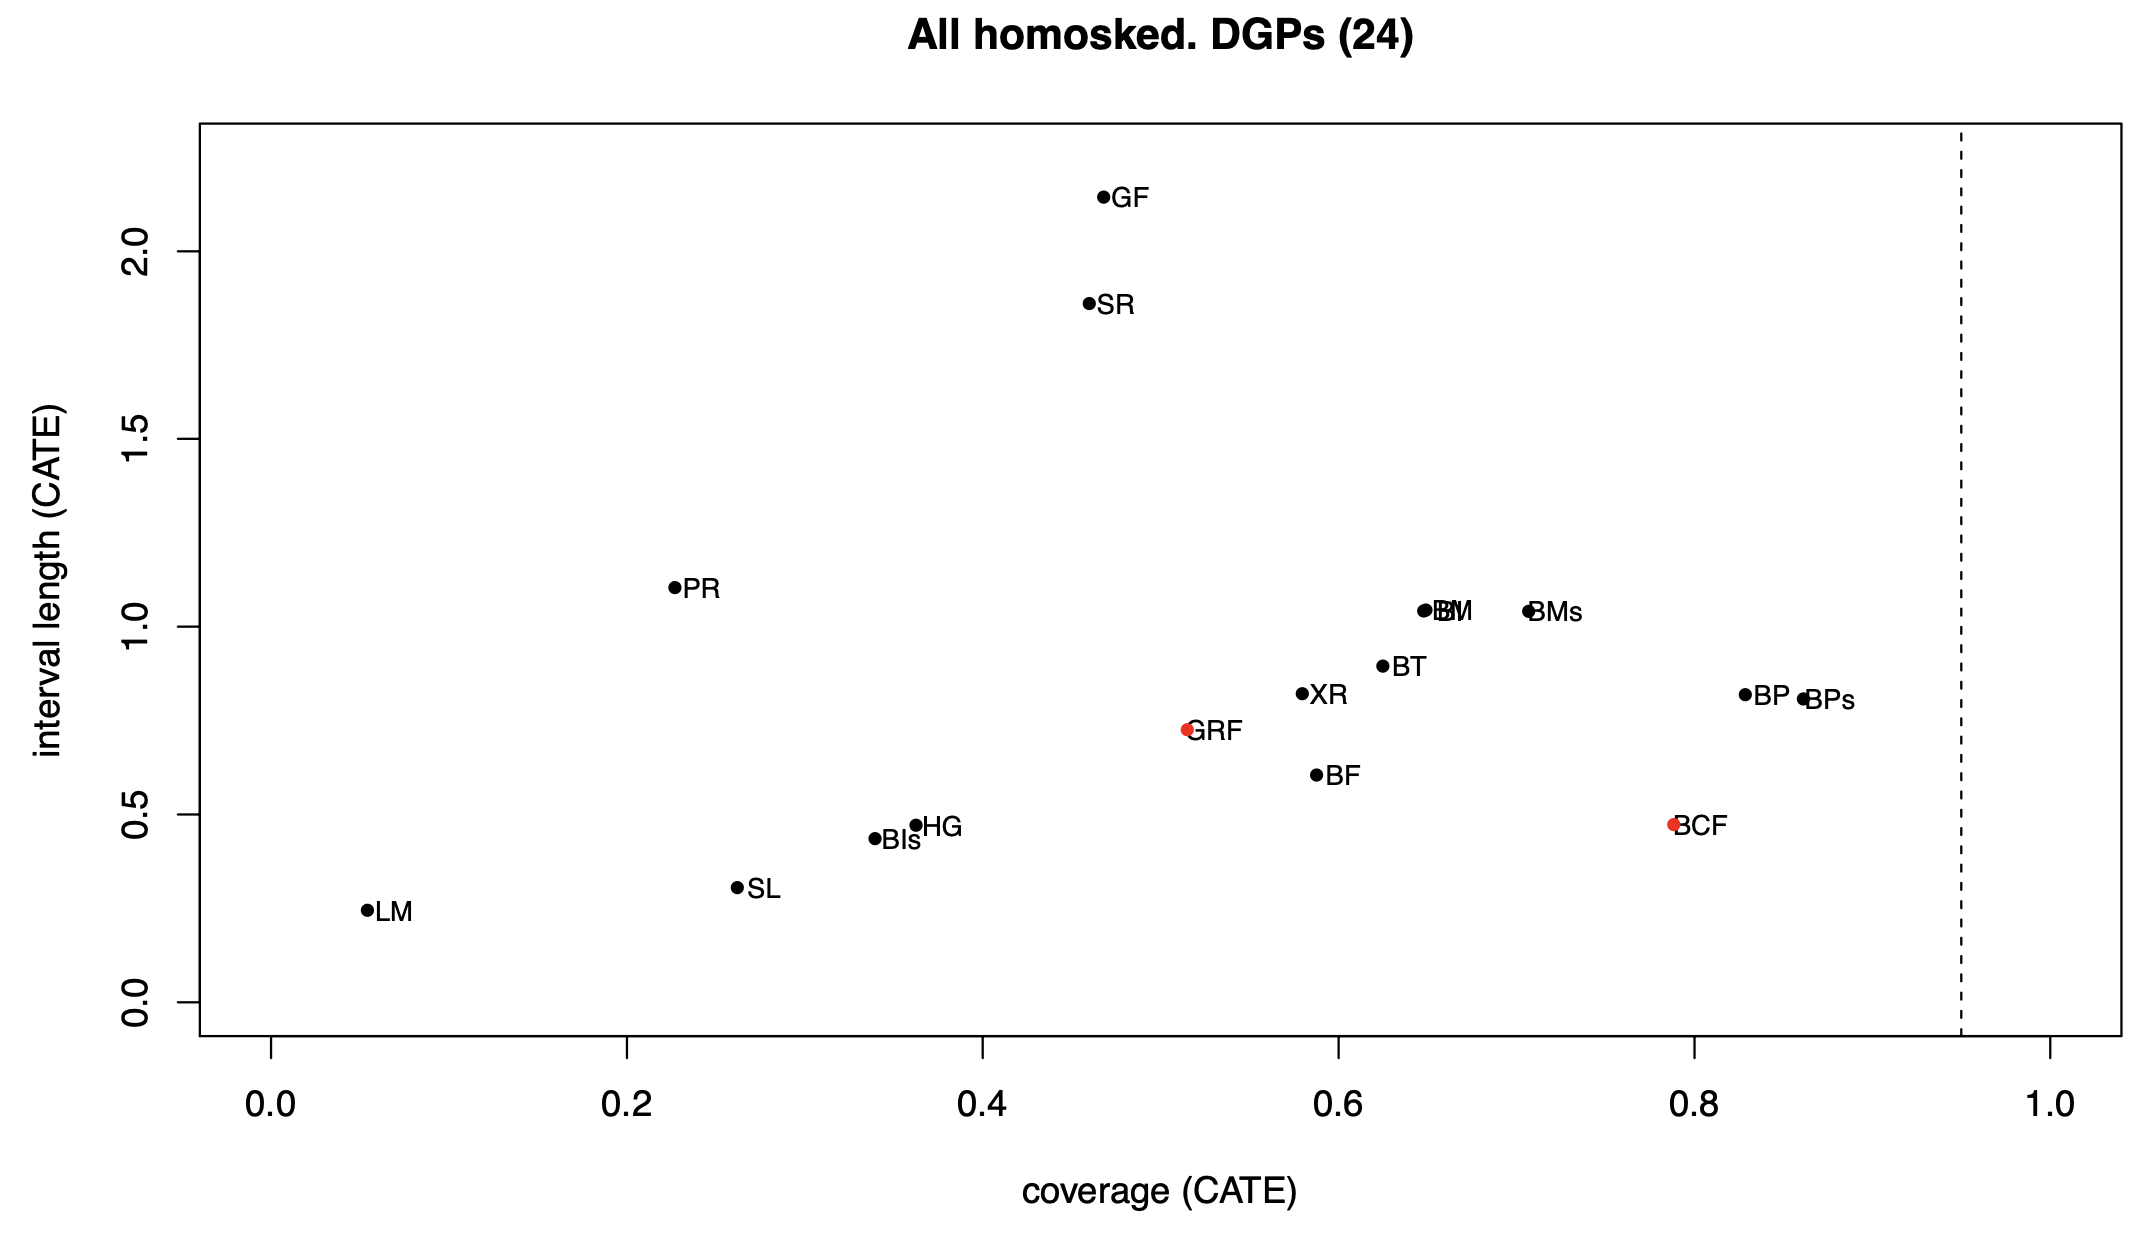
\includegraphics[scale=0.32]{figures/acic1}
	
\end{frame}

\begin{frame}
	\frametitle{ACIC 2017 {\small (data challenge for causal inference nerds)}}
	
	\hspace*{-8mm}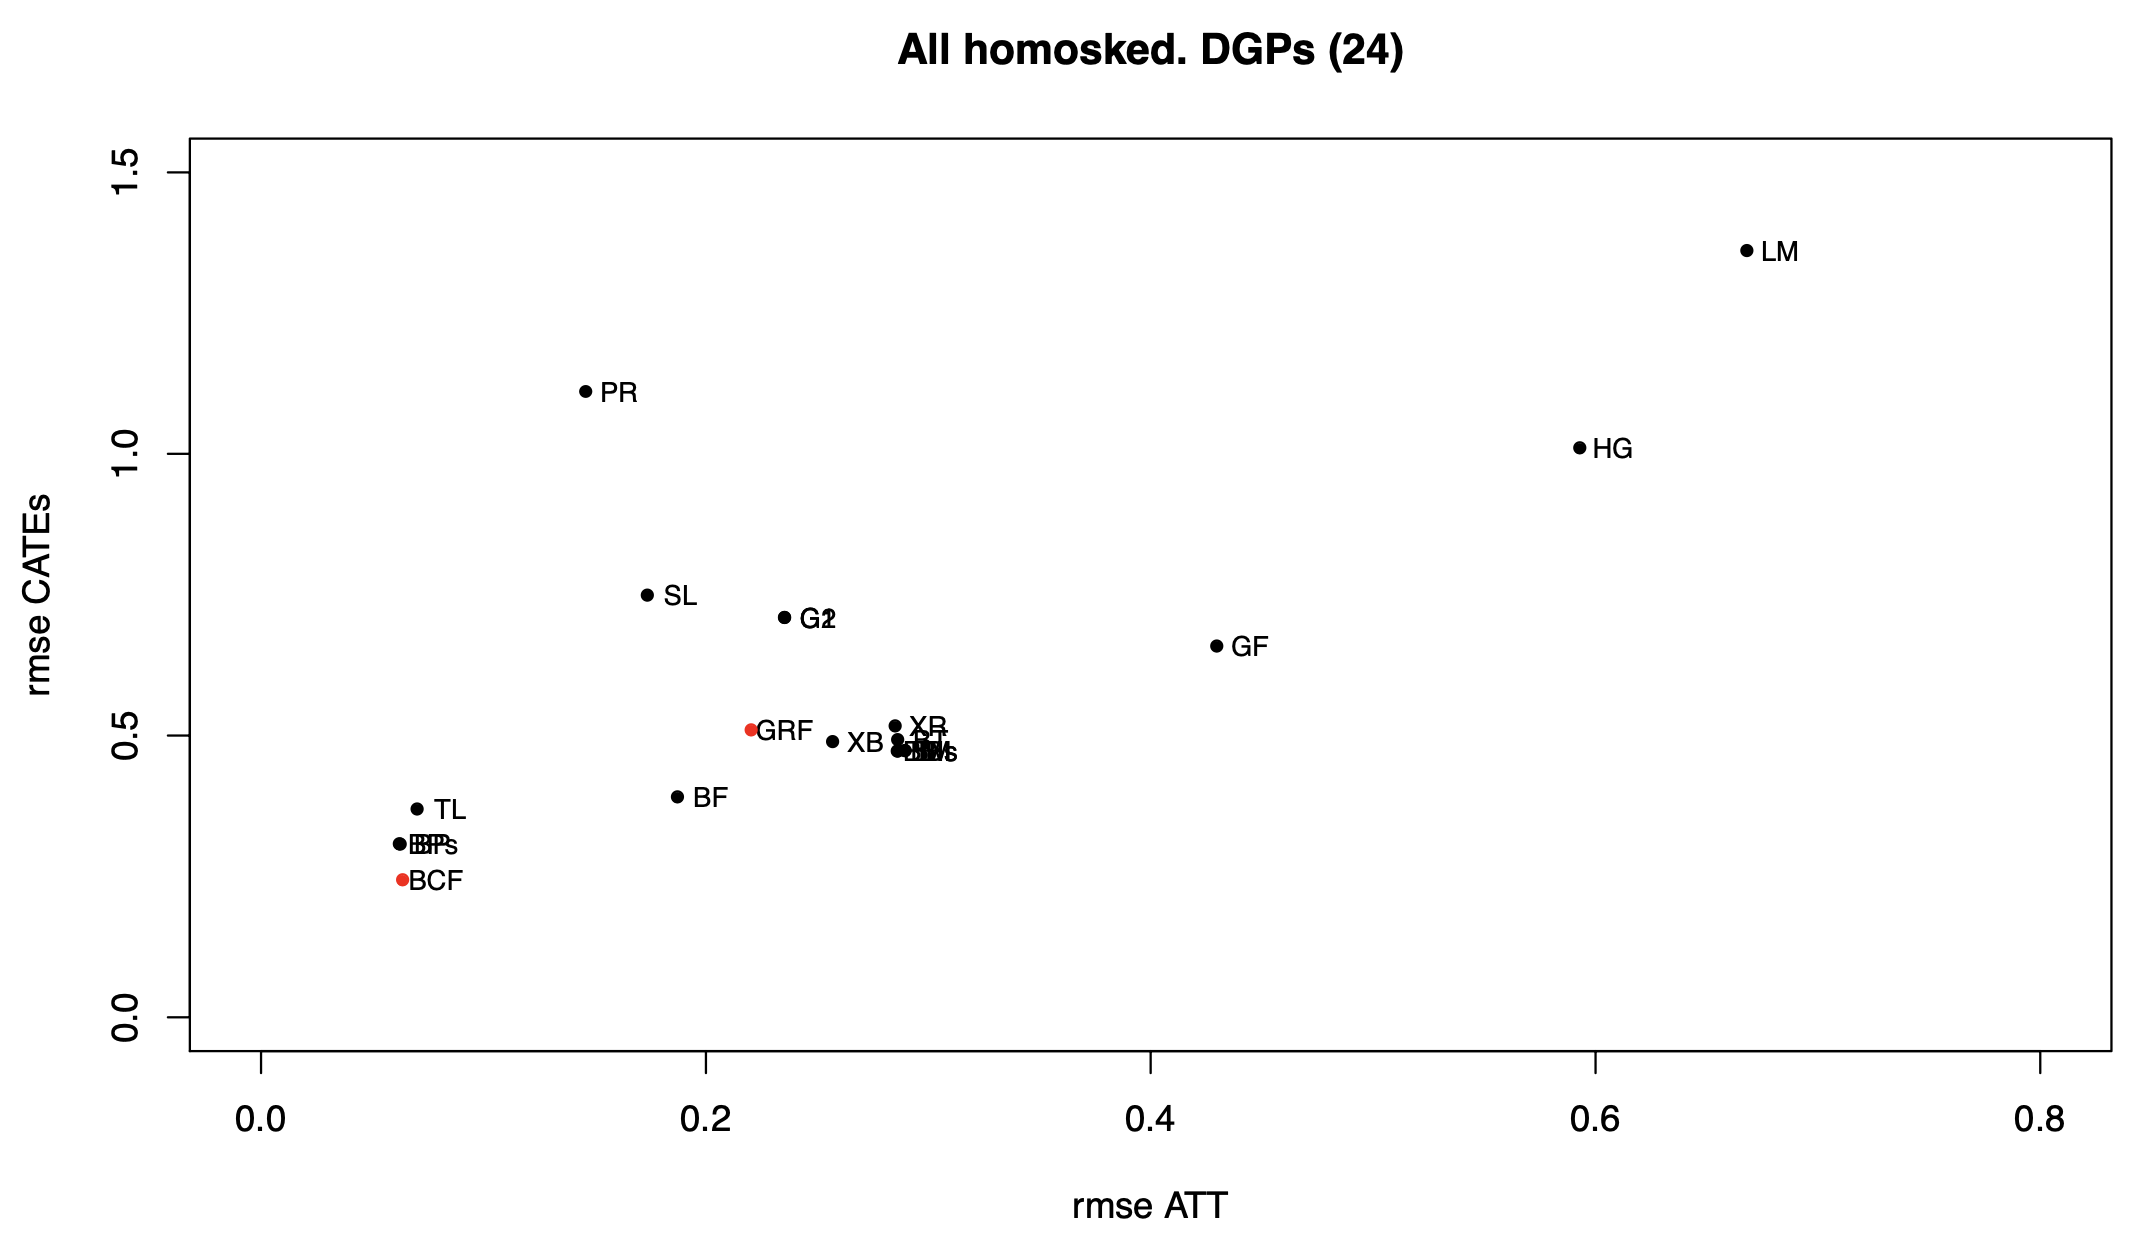
\includegraphics[scale=0.32]{figures/acic2}
	
\end{frame}


\begin{frame}
	\frametitle{Wrap up}
	
	\lb{Adjusting for confounding} is fundamentally different than estimating the best predictive model.
\vfill
\lb{Regularization} helps ``structure'' a complex model, but it has to be deployed in the right way for causal inference (propensity score adjustment, reparameterizations, ...)
\vfill
So much interesting work to do in this area, and it involves deeply understanding ML methods that were once only thought of as blackboxes.



\end{frame}


\end{document} 











